\documentclass[12pt]{article}

\usepackage{sbc-template}

\usepackage{graphicx,url}

%\usepackage[brazil]{babel}   
\usepackage[utf8]{inputenc}  

     
\sloppy

\title{MO446 - Visão Computacional\\Panoramas}

\author{Caio R. Teixeira \inst{1}, Carlos D. de L. Brasil \inst{2}, Flávio A. P. Cunha \inst{1}, Vitor de M. Calhau\inst{3} }


\address{Universidade Federal de Campinas
  (UNICAMP)\\
  Campinas -- SP -- Brazil
  \nextinstitute
  Instituto de Computação
  \email{\{c212661,c168296,f197083,v248740\}@dac.unicamp.br}
}

\begin{document} 

\maketitle

\section{Coleta das Imagens}

\section{Detecção e Extração de Características}
Pontos de interesse são aqueles que podem ser encontrado de forma confiável e consistente, mesmo sob a influência de diversas transformações da imagem, ou seja, o ponto de interesse deve ser detectado nas mesmas localizações físicas da cena, independente de mudanças no ponto de vista da cena, iluminação, ou outros fatores de ruído. Também cada ponto deve possuir uma aparência única em sua vizinhança imediata, permitindo que seja distinguido de outros pontos. Canto são bons exemplos,pois um canto é uma junção de duas ou mais bordas com direções diferentes. Esta ideia foi a base para um dos detectores mais clássicos e influentes: o detector de cantos de Harris, que foi visto em sala de aula.Mas para esse projeto veremos outros dois detectores de características, o SIFT e o ORB.

O SIFT (Scale-Invariant Feature Transform) é um algoritmo revolucionário em Visão Computacional, projetado para detectar e descrever características locais em uma imagem. Sua principal vantagem é ser invariante à escala, rotação e iluminação, além de parcialmente invariante a mudanças de ponto de vista.O SIFT primeiro procura por pontos potenciais de interesse em todas as escalas da imagem. Para isso, ele cria uma Pirâmide de Diferença de Gaussianas (DoG), e depois aplica uma Diferença de Gaussianas (DoG), assim ele consegue  procurar por máximos e mínimos locais  nessas imagens DoG.Um pixel é selecionado como ponto-chave candidato se for o maior ou o menor entre seus 8 vizinhos na mesma escala e os 9 vizinhos nas escalas acima e abaixo.

Porém nem todos os pontos candidatos são estáveis ou robustos o suficiente. O SIFT utiliza um processo de refinamento para eliminar pontos de baixo contraste (muito sensíveis ao ruído) ou pontos localizados ao longo de bordas (que são mal definidos e sensíveis a ruídos). Para alcançar a invariância à rotação, para cada ponto-chave é atribuída uma ou mais orientações dominantes com base nas características locais da imagem. Por fim , é criado um vetor descritor que captura de forma única a aparência da região ao redor do ponto-chave. A imagem \ref{fig:sift} mostra um exemplo de uma imagem com os pontos de características SIFT detectados.

\begin{figure}[ht]
    \centering
    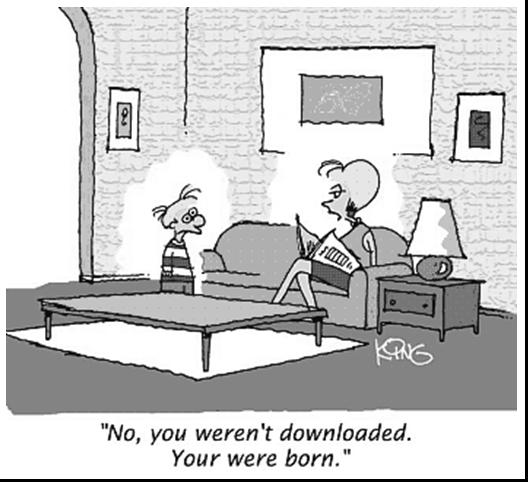
\includegraphics[width=0.5\textwidth]{sift.jpg}
    \caption{Pontos de características SIFT}
    \label{fig:sift}
\end{figure}

O ORB é um algoritmo detector e descritor de características (pontos de interesse) em imagens que se tornou extremamente popular por combinar eficiência e bom desempenho, por ser alternativa livre de royalties e mais rápida ao algoritmos SIFT, o ORB é composto por duas partes principais: um detector para encontrar os pontos e um descritor para caracterizá-los.

O ORB usa o detector FAST (Features from Accelerated Segment Test) para encontrar pontos de interesse, ele identifica pontos candidatos verificando se um círculo de 16 pixels ao redor de um pixel central possui um número contíguo de pixels significativamente mais claros ou mais escuros que o ponto central. O ORB usa o descritor BRIEF (Binary Robust Independent Elementary Features), para caracterizar os pontos, ele funciona criando um vetor de bits (0s e 1s) através de uma série de testes simples de intensidade entre pares de pixels pré-definidos em uma região ao redor do ponto. A imagem \ref{fig:orb} mostra um exemplo de uma imagem com os pontos de características ORB detectados. 

\begin{figure}[ht]
    \centering
    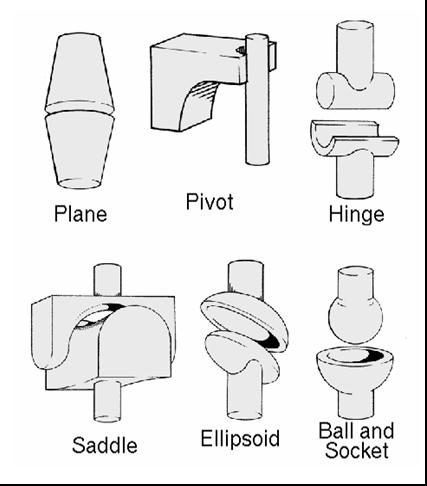
\includegraphics[width=0.5\textwidth]{orb.jpg}
    \caption{Pontos de características ORB}
    \label{fig:orb}
\end{figure}

Fora utilizados esses dois descritores pois o ORB é um  detector-descritor robusto, rápido e prático, enquanto o SIFT  é um descritor altamente robusto para cada ponto-chave, permitindo que correspondências confiáveis sejam encontradas entre imagens mesmo sob condições drasticamente diferentes.

\section{Emparelhamento de Características}

O objetivo desta etapa foi descobrir quais keypoints de uma imagem correspondem aos da outra imagem. Esse processo é extremamente importante, visto que a construção de um bom panorama final depende do alinhamento correto das regiões correspondentes entre as imagens. 

Após obter os descritores das features na etapa passada (através dos dois detectores usados, SIFT e/ou ORB), é preciso comparar os descritores de cada imagem. Para fazer isso, pode-se utilizar diferentes abordagens, como Brute Force e FLANN. Para este trabalho, foram testadas ambas as técnicas: para a primeira versão foi usado Brute Force, enquanto que para o teste de composição automática do panorama, foi utilizado uma versão semelhante à FLANN, mas fazendo uso da função cKDTree, de spicy.spatial, em vez da abordagem pronta do OpenCV.

O resultado dos algoritmos de emparelhamento é um conjunto de correspondências candidatas entre os keypoints, mas que pode ter muitos outliers, ou seja, correspondências falsas. Por isso, existe a necessidade de aplicar filtros, sendo um deles o Ratio Test. Essa técnica verifica, para cada descritor de uma imagem, os dois descritores mais próximos na outra imagem. Se a razão da distância do melhor desses dois para o segundo melhor for menor que um threshold, ele é considerado como uma boa correspondência. Isso tenta filtrar pegando apenas os candidatos que estão muito mais próximos do que o segundo melhor, evitando aqueles com ambiguidades.

Por fim, depois de obter apenas as melhores correspondências, foi aplicado uma técnica para visualização das mesmas, com o intuito de verificação e validação. Para isso, usou-se a função \texttt{drawMatches()}, da biblioteca OpenCV.
Durante os primeiros testes nessa etapa de emparelhamento de características, foram observadas dificuldades ao trabalhar com imagens que apresentavam pouca sobreposição ou regiões de baixa distinção visual, especificamente fotos tiradas em ambientes naturais, com predominância de árvores. Nessas situações, o número de correspondências confiáveis foi insuficiente para estimar corretamente a homografia, o que mostrou-se nas etapas seguintes, mas teve raiz nessa etapa. Por isso, posteriormente, foi necessário buscar outras imagens, com maior sobreposição e distinção.

\section{Estimação de Homografia e Alinhamento}

É necessário encontrar os pontos estáticos certos para computar a pose e consequentemente o alinhamento entre casamento destes pontos em imagens distintas. Para encontrar o melhor casamento dentre os pares encontrados no passo anterior de matching, utilizamos como abordagem o RANSAC ( Random Sample Consensus ) para cálculo da matriz homografia H.

RANSAC é um algoritmo iterativo para ajustar modelos lineares que é robusto a outliers. Essa robustez se deve ao fato de que o algoritmo estima os parâmetros baseado apenas em um subconjunto de pontos identificados como inliers dos dados.

Este cuidado com a qualidade dos dados é importante pois a matriz de homografia inferida é sensível a ruídos nos dados e a maus casamentos entre os pixels.

Uma vez estimada a Homografia, precisaremos aplicar uma transformação (warp) em uma das imagens mapeando-a em um plano comum. Assim, aplicamos uma transformação de perspectiva, que combina operações de rotação, escala e translação, a {imagem da direita} de modo a combinar as imagens. Para tanto, usamos a função \texttt{warpPerspective()} implementada na biblioteca OpenCV que transforma a imagem de origem usando a matriz de Homografia calculada. 

\section{Composição e Blending}

\subsection{Processo de Montagem do Panorama}
A montagem do panorama final é um processo que envolve a combinação precisa de múltiplas imagens em uma única cena contínua. Após o alinhamento geométrico das imagens através da homografia, é necessário garantir uma transição suave nas regiões de sobreposição para evitar descontinuidades visuais. Este processo é particularmente desafiador devido a variações de exposição, diferenças de iluminação e pequenos erros de alinhamento entre as imagens.

\subsection{Blending}
O blending é uma etapa crucial na criação de panoramas por várias razões:
\begin{itemize}
    \item \textbf{Suavização de transições}: Elimina bordas visíveis entre as imagens sobrepostas
    \item \textbf{Compensação de variações de exposição}: Minimiza diferenças de brilho e contraste entre as imagens
    \item \textbf{Redução de artefatos}: Esconde pequenos desalinhamentos residuais após a transformação geométrica
    \item \textbf{Integração natural}: Cria uma aparência contínua e natural na cena final
\end{itemize}

\subsection{Implementação do Alpha Blending}
A técnica de \textit{alpha blending} implementada utiliza uma abordagem baseada em pesos que variam de acordo com a distância de cada pixel até as bordas da imagem. O processo ocorre em três estágios principais:

\begin{enumerate}
    \item \textbf{Geração de máscaras de peso}:
    \begin{itemize}
        \item Cada imagem é convertida para escala de cinza e limiarizada para criar máscaras binárias
        \item Um mapa de distância é calculado para cada máscara, onde o valor de cada pixel representa sua distância até a borda mais próxima
    \end{itemize}
    
    \item \textbf{Normalização dos pesos}:
    \begin{itemize}
        \item Os mapas de distância são normalizados para criar funções de peso que variam suavemente de 0 a 1
        \item A normalização garante que a soma dos pesos correspondentes de todas as imagens seja igual a 1 em cada ponto
    \end{itemize}
    
    \item \textbf{Combinação ponderada}:
    \begin{itemize}
        \item Cada canal de cor é ponderado de acordo com os mapas de peso calculados
        \item A imagem final é formada pela soma ponderada das imagens alinhadas
    \end{itemize}
\end{enumerate}

\subsection{Análise dos Resultados}
A implementação atual apresenta as seguintes características:

\begin{itemize}
    \item \textbf{Pontos Fortes}:
    \begin{itemize}
        \item Transições suaves entre imagens devido ao alpha blending
        \item Tratamento automático de sobreposições
        \item Remoção de bordas pretas através da função \texttt{auto\_crop}
    \end{itemize}
    
    \item \textbf{Desafios Encontrados}:
    \begin{itemize}
        \item Dificuldade em regiões com poucas características distintas
        \item Possíveis desalinhamentos em cenas com objetos em movimento
        \item Sensibilidade a variações de iluminação entre as imagens
    \end{itemize}
\end{itemize}

A função \texttt{auto\_crop} é responsável por remover as bordas pretas resultantes da composição, utilizando detecção de contornos para identificar a região de interesse e recortar a imagem final de forma adequada.

\bibliographystyle{sbc}
\bibliography{sbc-template}

\end{document}
